\scanpage{231}
\margin{\diagram{\begin{tikzcd}S\arrow[d]\\T\end{tikzcd}}}
\unsure{version relatif}
\margin{\figure{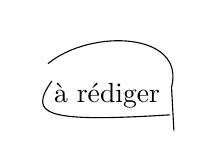
\begin{tikzpicture}[baseline=(n.base)]\node(n) at (0,0){\unsure{à rédiger}};\draw (0.85,-0.45)--(0.82,0.1) .. controls (1,0.8) and (-0.2,0.85) .. (-0.75,0.4);\draw (-0.7,0.18) .. controls (-1,-0.25) and (-0.8,-0.35) .. (0.8,-0.25);\end{tikzpicture}}}

1) Soit
\diagram{\begin{tikzcd}F\arrow[r,"D"]&G\arrow[r,"D'",no head]&H\end{tikzcd}}
une suite d'op. différentiels, qui est ``formellement exacte''. Alors pour tt $P$, la suite
\diagram{\begin{tikzcd}
\operatorname{Diff}^i(P,F)\arrow[r,"u\mapsto D\circ u"]&
\operatorname{Diff}^{i+1}(P,G)\arrow[r,"v\mapsto D'\circ v",no head]&
\operatorname{Diff}^{i+2}(P,H)
\end{tikzcd}}
est exacte, et la suite
\diagram{\begin{tikzcd}
\operatorname{Diff}^i(H,P)\arrow[r,"u\mapsto u\circ D'"]&
\operatorname{Diff}^{i+1}(G,P)\arrow[r,"u\mapsto u\circ D"]&
\operatorname{Diff}^{i+2}(F,P)
\end{tikzcd}}
est exacte.

2) Supposons que $E$ sur $S$ soit loc. libre \uline{stratifié}, et que le lemme de Poincaré formel soit vrai pour le complexe
\[
E\otimes\Omega^*_{S/T}=\Omega^*_{S/T}(E)
\]
[p.ex. $S$ lisse sur $T$, et caractéristiques de $T$ nulles].
Alors \inserted{$\forall\ P$ quelc. et $i\geq0$} la suite
\diagram{\begin{tikzcd}[column sep=large]
0 & \operatorname{Hom}(E,P)\arrow[l] &
\operatorname{Diff}^i(E,P)\arrow[l,"\deleted{\unsure{u\mapsto u(h)}}"']\arrow[d,"\sim"'] &
\operatorname{Diff}^{i-1}(\unsure{E}\otimes\Omega^1_{S/T},P)\arrow[l,"u\mapsto u\circ d_E^0"'] &
\cdots\arrow[l,"u\mapsto u\circ d_E^1"']\\
&\bigl[&\operatorname{Hom}(P^i(E),P)\arrow[ul,"u\mapsto u\circ\unsure{\delta_i^E}"']&\bigr]
\end{tikzcd}}
\inserted{où $\unsure{\delta_i^E}:E\to P^i(E)$ défini par la stratification}
est exacte.

\uline{NB} $\operatorname{Ker}(\operatorname{Diff}^i(E,P)\to\operatorname{Hom}(E,P))$ est désigné par
$\operatorname{Diff}^i_+(E,P)$, op. diff. ``à coeff. cts'' rel. à la stratification.
\margin{230}
